\chapter{Caches}
\section{Why Caches}
The difference between cycle time (time of a stage in a pipeline) and memory access time has continually increased.
\begin{center}
    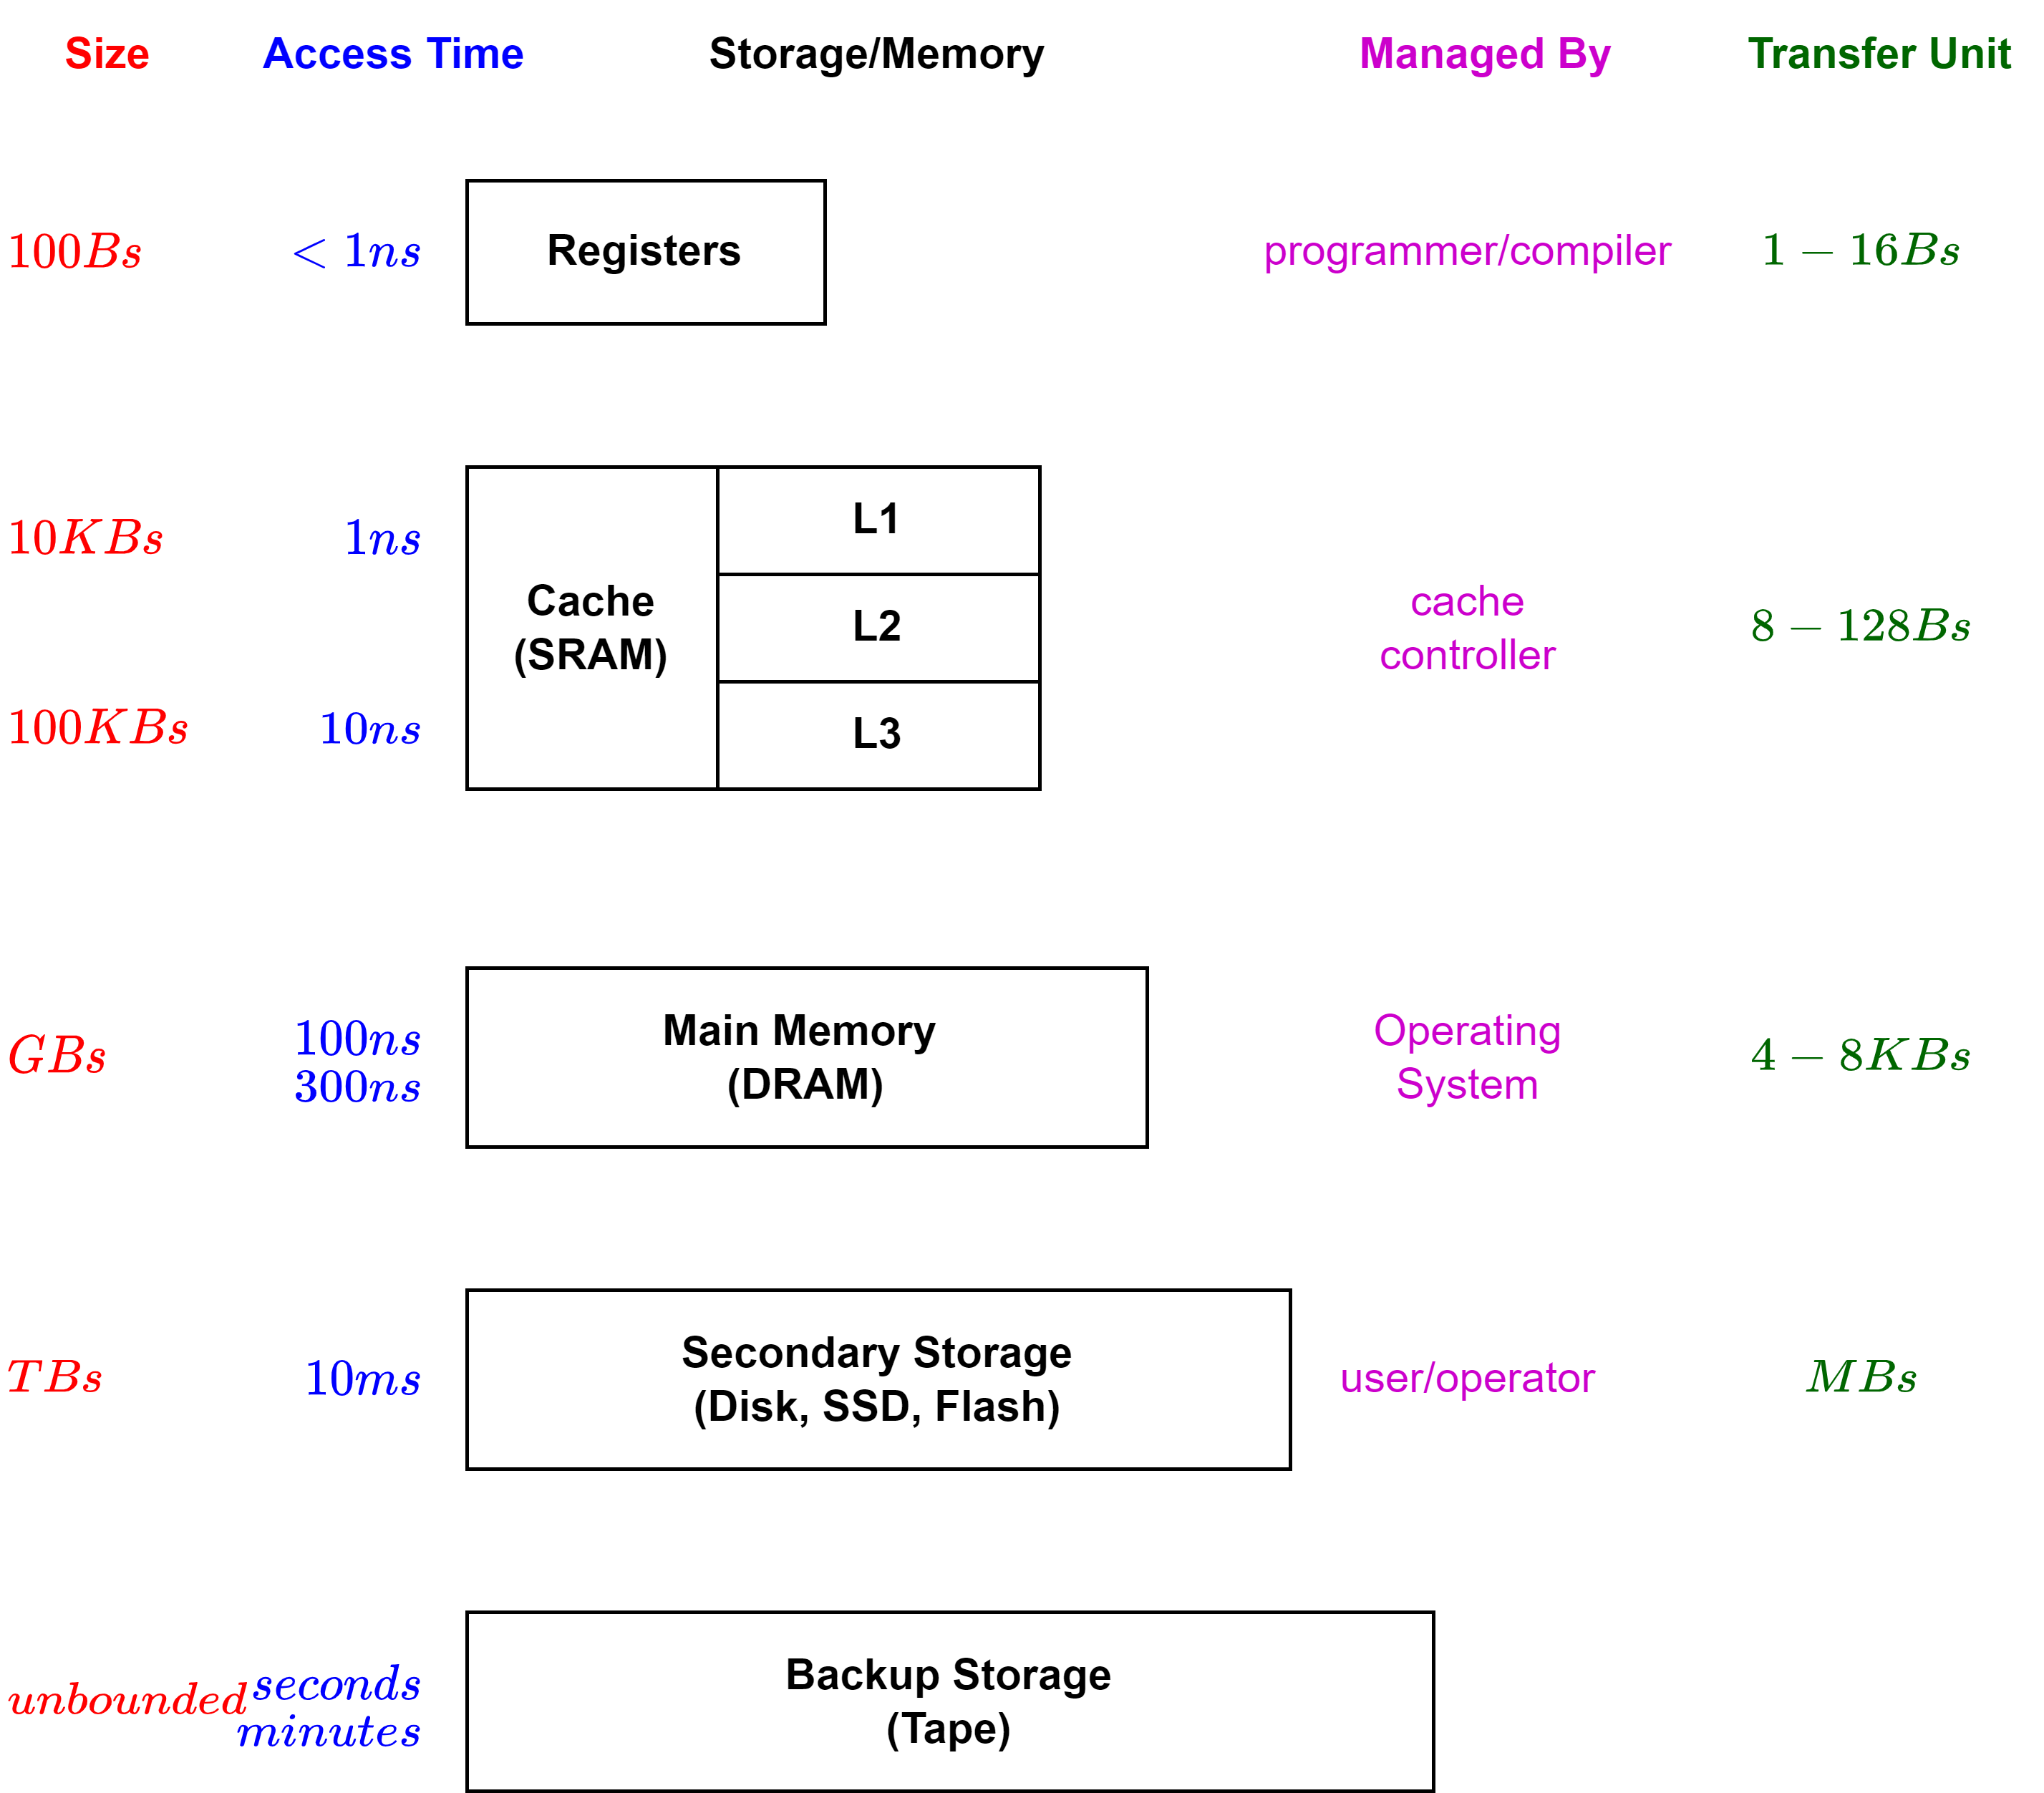
\includegraphics[width=.9\textwidth]{caches/images/memory_hierarchy.drawio.png}
\end{center}
\section{Locality}
Programs typically access only a small part of their address space during a short time period.
\begin{tcbraster}[raster columns=2,raster equal height]
    \begin{definitionbox}{Temporal Locality}
        Locality in time. The same location referenced is often referenced multiple times.
    \end{definitionbox}
    \begin{definitionbox}{Temporal Locality}
        Locality in space. Locations near an accessed location tend to be referenced soon.
    \end{definitionbox}
\end{tcbraster}
Most modern architectures are reliant on locality to determine when and what locations should be cached.
\begin{itemize}
    \item Cache is a scarce resource.
    \item Cache misses are expensive.
\end{itemize}

\section{Cache Types}
\subsection{Directly Mapped Cache}
\begin{definitionbox}{Associativity Conflicts}
    Where two or more locations are mapped to the same cache line/set of cache lines, and repeatedly replace each other.
    \begin{minted}{C}
/* Example with arrays, assume cache line is 256 bytes
 * and both arrays start at same cache index 
 */

int array_a[64];
int array_b[64];

int some_function() {
    int sum = 0;
    for (int i = 0; i < 64; i++) {
        r += 
        array_a[i]    /* array_a moved into cache line */
        + array_b[i]; /* array_b evicts array_a and replaces */
    }
    return sum;
}
    \end{minted}
\end{definitionbox}

\begin{center}
    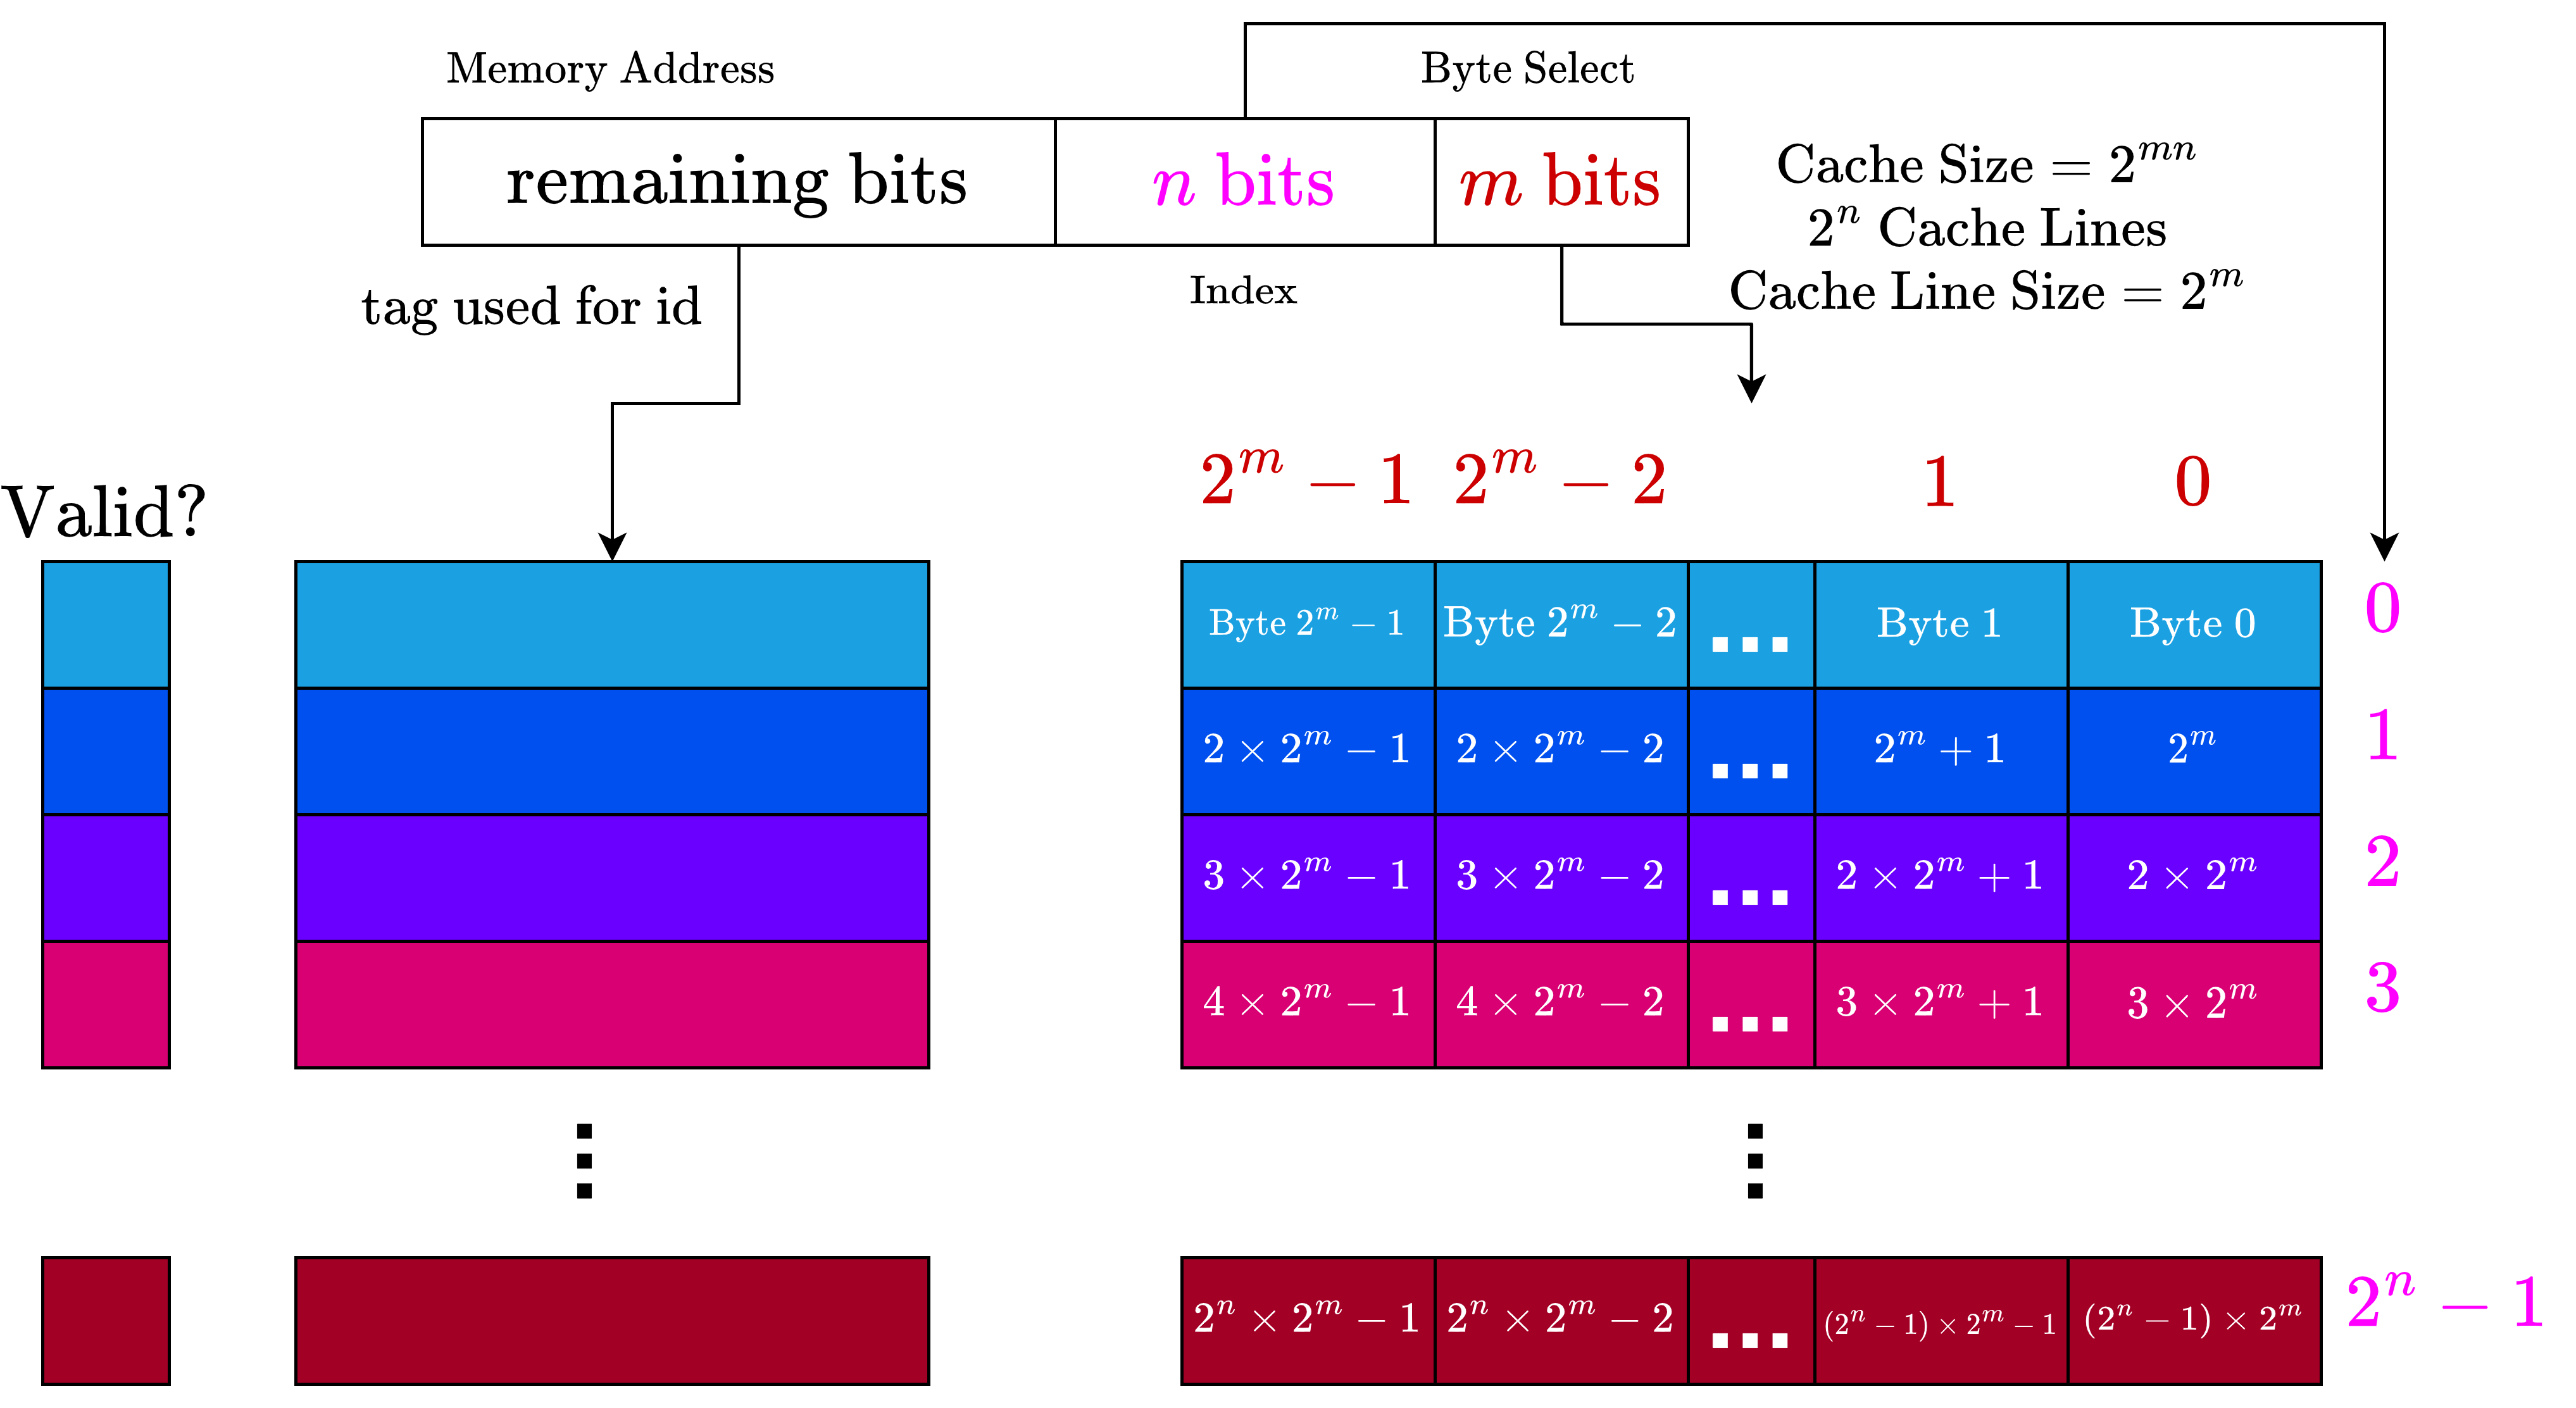
\includegraphics[width=.9\textwidth]{caches/images/direct_mapped_cache.drawio.png}
\end{center}
\begin{itemize}
    \item Index and byte select used to find entry. Then tag compared to determine hit/miss.
    \item We can see a pattern in memory of where locations can be cached based on the index.
    \item Block/line received before the hit/miss is known (recover later if miss).
\end{itemize}
\begin{center}
    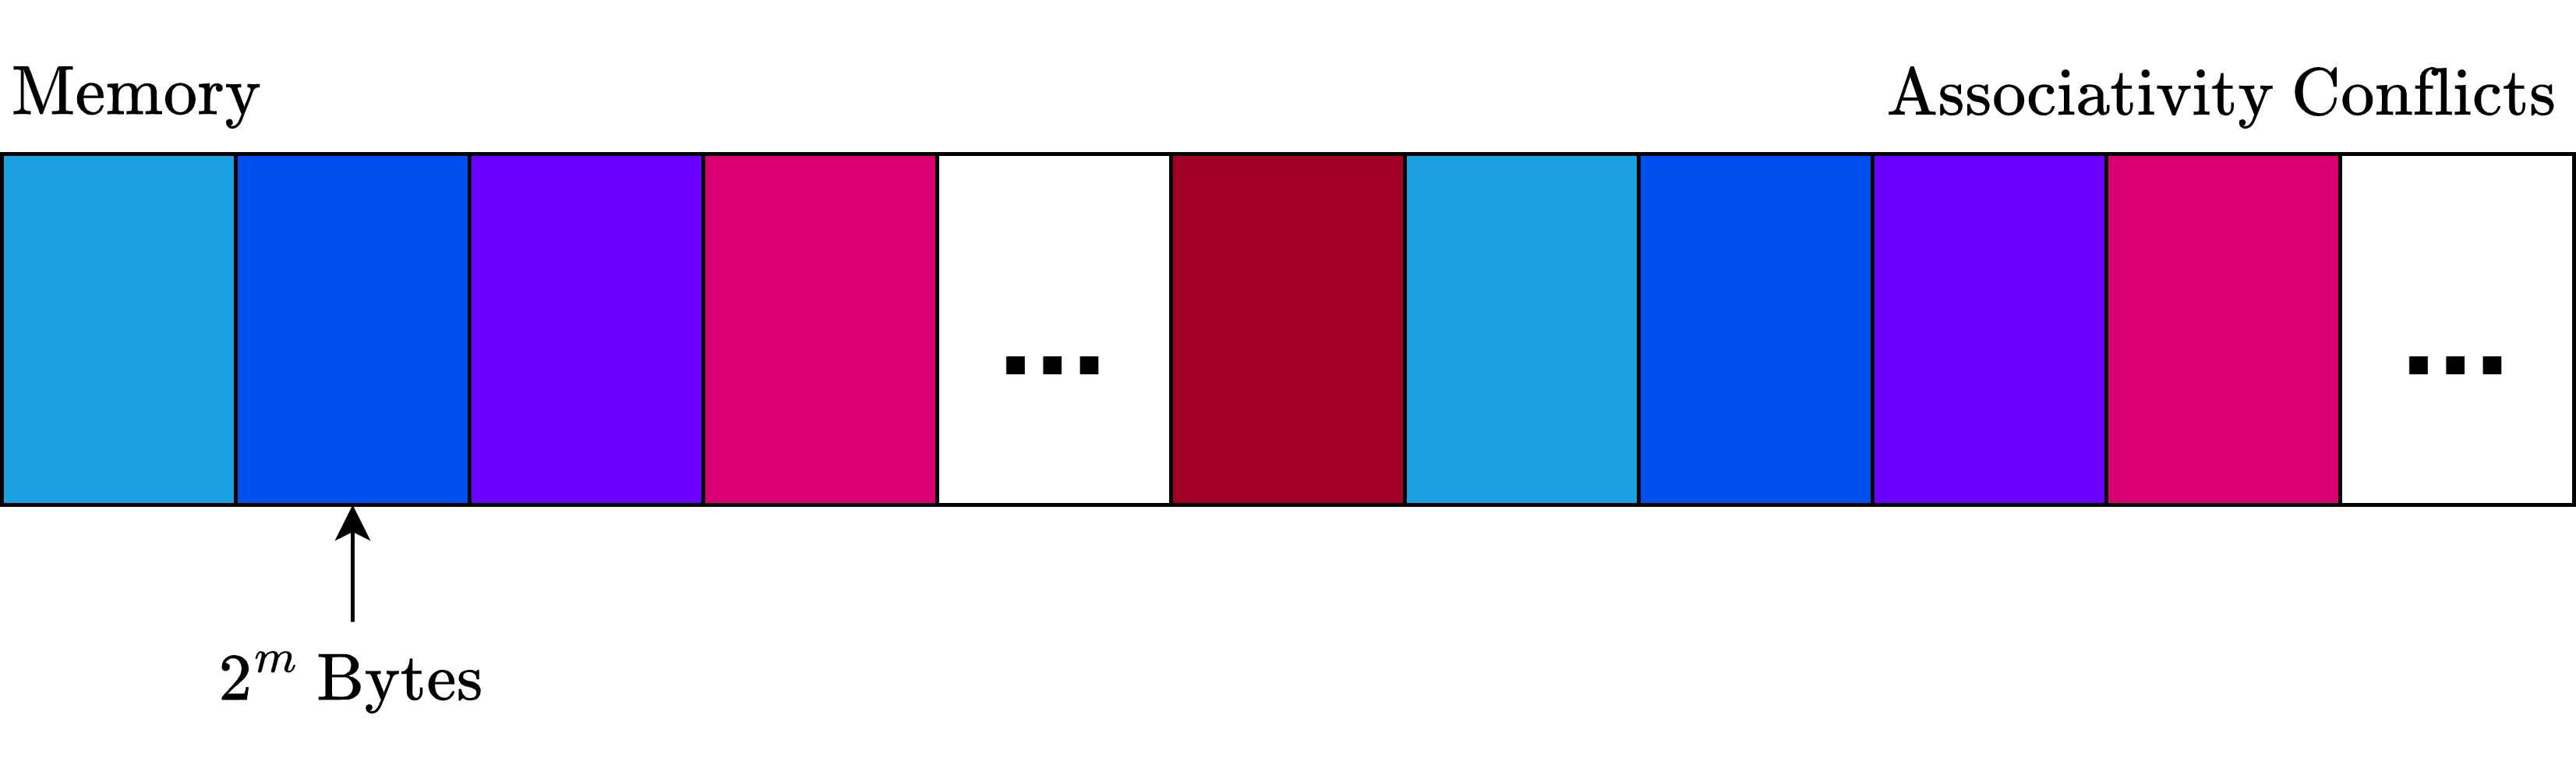
\includegraphics[width=.9\textwidth]{caches/images/associativity_conflicts.drawio.png}
\end{center}
\begin{prosbox}
    \begin{center}
        \begin{tabular}{r p{.8\textwidth}}
            \textbf{Simplicity} & Simple indexing of cache \& compare to determine hit/miss. \\
            \textbf{Fast Lookup} & Only one location where a cached value may be. \\
        \end{tabular}
    \end{center}
\end{prosbox}
\begin{consbox}
    \begin{center}
        \begin{tabular}{r p{.8\textwidth}}
            \textbf{Associativity Conflicts} & As location can only be cached in one place, associativity conflicts are common. \\
        \end{tabular}
    \end{center}
\end{consbox}

\subsection{Two Way Associative}
Combine two directly mapped caches, and only cache a given location in one.
\begin{center}
    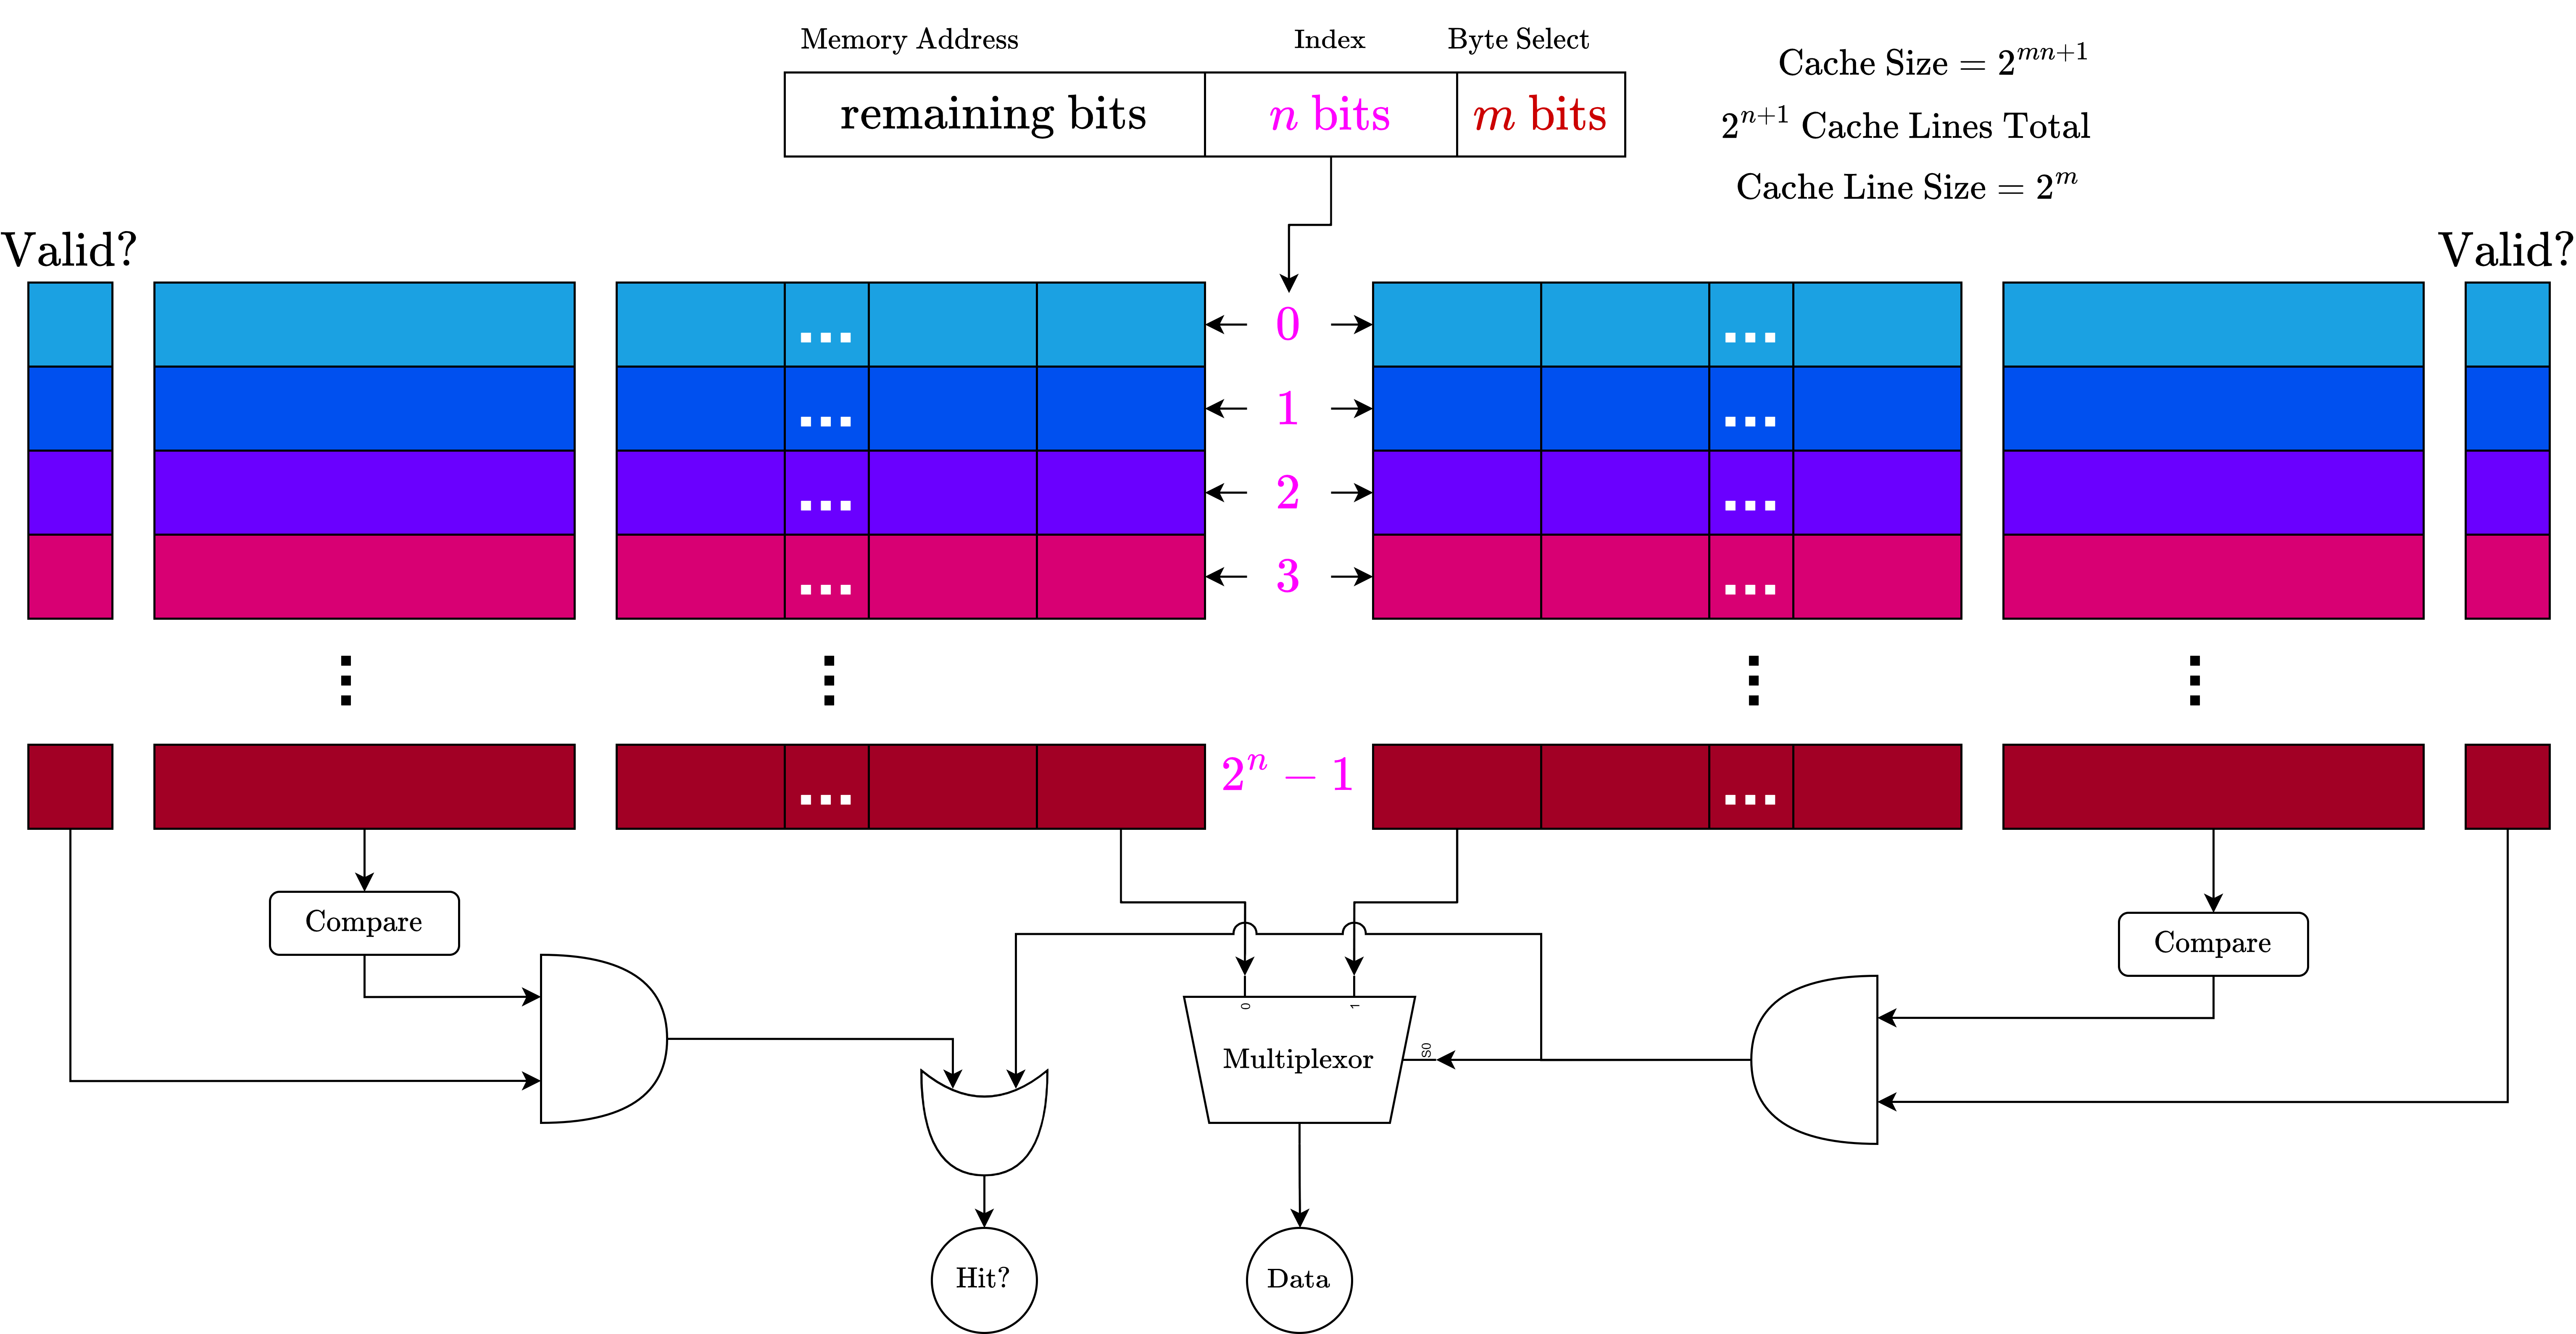
\includegraphics[width=.9\textwidth]{caches/images/two_way_set_associative.drawio.png}
\end{center}
\begin{itemize}
    \item Both caches searched in parallel.
    \item Only one hit possible, this is selected from result of both caches (selection is in the critical path)
    \item Cache block/line is available after the hit/miss is determined.
\end{itemize}

\begin{prosbox}
    \begin{center}
        \begin{tabular}{r p{.8\textwidth}}
            \textbf{Fewer Assoc Conflicts} & Any location can now select two different locations in the cache, hence two addresses with the same index can both be cached. \\
            \textbf{}
        \end{tabular}
    \end{center}
\end{prosbox}
\begin{consbox}
    \begin{center}
        \begin{tabular}{r p{.8\textwidth}}
            \textbf{Multiplexer Delay} & A multiplexer is added in the critical path \\
            \textbf{Complexity} & Requires more comparators, and more complexity in placement \& replacement. \\
        \end{tabular}
    \end{center}
\end{consbox}

\subsection{N Way Associative \& Block Placement}
A generalisation of the directly mapped and two way associative caches. Block placement is restricted by the cache's associativity.
\begin{itemize}
    \item Increasing associativity reduces associativity conflicts $\Rightarrow$ better hit rate (with diminishing returns)
    \item Greater overhead in terms of multiplexers in the critical path and the hardware complexity
    \item Fully associative cache can place any location in any cache location, and uses parallel search of tag (index is $0$ bits) to find entry
    \item More associative $\Rightarrow$ less sensitivity to storage layout
\end{itemize}
\begin{sidenotebox}{Intel Pentium 4 Level 1 Cache (pre-prescott)}
    \begin{center}
        \begin{tabular}{r l | r l}
            \textbf{Capacity:} & $8KB$ & \textbf{Block/Line Size:} & $64B$ so $\sfrac{8K}{64} = 128$ blocks\\
            \textbf{Ways/Associativity:} & $4$ & \textbf{Sets:} & $32$ ($128$ blocks, but $4$ way $\Rightarrow \sfrac{128}{4}$) \\
            \textbf{Index:} & $5$ bits & \textbf{Tag:} & $21$ bits \\
        \end{tabular}
    \end{center}
    Resulting access time is $2$ cycles ($6ns$ at $3GHz$), with cache/memory being dual ported (load and store).
\end{sidenotebox}

\section{Block Identification}
Index and tag identify a block.
\begin{itemize}
    \item Increasing associativity decreases index size, increases tag size.
    \item Increasing block size decreases index size.
\end{itemize}

\section{Block Replacement}
When introducing a new location to the cache \& possible locations are full.
\begin{itemize}
    \item No choice in directly mapped.
    \item $n$ choices for $n$-way associative.
\end{itemize}
The least recently used (LRU) evicts the oldest cache entry
\begin{itemize}
    \item In practice only a marginal advantage over random eviction.
    \item Can be pathologically bad (e.g a loop accessing many locations may evict the first just before restarting the loop \& accessing again).
\end{itemize}

\section{Write Strategy}
\begin{tcbraster}[raster columns=2, raster equal height]
    \begin{definitionbox}{Write Through}
        Write to cache, and to the block in lower-level memory.
        \begin{itemize}
            \item Combined with write buffers to prevent a wait on memory
        \end{itemize}
    \end{definitionbox}
    \begin{definitionbox}{Write Back}
        Only write back when evicting from cache. 
        \begin{itemize}
            \item Track write backs with a dirty bit
            \item Absorb cost of repeated writes
        \end{itemize}
    \end{definitionbox}
\end{tcbraster}
Neither avoid the cache-coherence problem (inconsistent values for locations cached on multiple cores/processors).
